\documentclass[a4paper, 11pt]{article}

\usepackage[T1]{fontenc}
\usepackage[utf8]{inputenc}
\usepackage[spanish]{babel}
\usepackage{graphicx}

\usepackage{microtype}

\usepackage{xcolor}

\title{Aprendizaje Automático \\ Trabajo Práctico 1 --- Detección de Spam}
\author{Martín Fixman \and Leandro Matayoshi \and Fernando Gasperi}
\date{Segundo Cuatrimestre de 2016}

\newcommand{\todox}{\(\mathit{\color{red}x}\)}

\newcommand{\ham}{\large{\texttt{ham}}}
\newcommand{\spam}{\large{\texttt{spam}}}

\begin{document}
\maketitle

\newpage

\section{Extracción de Atributos}

\subsection{Análisis de texto}

Para obtener atributos relacionados con análisis de texto decidimos trabajar específicamente con 2 campos: \(body\) y \(subject\).

La extracción se realizó en base a aplicar Bayes sobre la probabilidad de que un mensaje sea \spam{} dada la aparición de una palabra (potencial atributo) en dicho mensaje.

Sea $w \in W$, siendo $W$ el universo de palabras obtenido a partir de los mails utilizados para entrenar el modelo.

\vspace{5px}
$P(spam \vert w) = \frac{P(w \vert spam) \cdot P(spam)}{P(w)}$, donde:

\vspace{5px}
$P(w \vert spam) = \frac{\sum_{s \in spam}^{} w \in s}{\mid spam \mid}$, $P(w) = \frac{\sum_{m \in M}^{} w \in m}{\mid M \mid}$, $P(spam) = \frac{\mid spam \mid}{\mid M \mid}$

\vspace{5px}
Análogamente, se realiza la misma operación para analizar las palabras que aparecen en los mails de \ham{}.

El primer experimento consistió en encontrar las 100 palabras que aparezcan en el body de los mails, y que maximicen el valor de Bayes tanto para \spam{} como
para \ham{}. Dicho de otra forma, encontramos las 100 palabras más spammeras y las 100 palabras más hammeras que aparezcan en el \(body\) de los mails.

Posteriormente realizamos un segundo experimento, repitiendo el proceso para las palabras del \(subject\) de los mails.

Durante esta etapa utilizamos la clase \(CountVectorizer\) del módulo \(feature \ extraction\) de \(sklearn\). \(CountVectorizer\) admite como parámetro un token-pattern,
que determina la estructura que deben seguir las palabras analizadas para ser consideradas potenciales features. En este caso, luego de probar con varios valores, optamos
por elegir palabras que contengan solo caracteres entre [a-z], y de longitud mínima = 4. Al mismo tiempo, también admite un parámetro que determina
la cantidad mínima de apariciones que debe tener una palabra para ser considerada \(token\). En este caso, luego de probar con varios valores, determinamos los valores de
800 apariciones para el caso del \(body\) y 200 para el \(subject\). Es decir, solo las palabras que aparecen como mínimo esa cantidad de veces entre la totalidad de
los mails fueron consideradas como tokens.


\section{Selección de Modelos}

En el punto anterior logramos conseguir una \textbf{Matriz de Features} \( X \), con \todox{} columnas (features) y \todox{} filas (samples), y un vector de clases \( y \) con \todox{} samples, donde cada una índica si cada sample debería pertenecer a \ham{} o a \spam{}. Dadas estos datos, vamos a elegir varios modelos que pueden lograr seleccionar el modelo óptimo para la inferencia.

\subsection{Metodología de Puntaje}

A cada modelo presentado se le asigna un \textbf{puntaje}, que indica cuán bien este predijo la categoría de cada mails con features similares a \( X \). Para prevenir los casos de overfitting, se usa \textbf{Stratified K-Folds} validation como validación cruzada, eligiendo un valor de \( k = 10 \)\footnote{Este valor nos pareció un poco elevado para este caso, pero este es el más comunmente usado}. De esta manera, tomamos el puntaje final como el puntaje promedio de los folds.

Adicionalmente, todos los modelos que requieran algo de azar se ejecutan con la misma raíz (\texttt{random\_state es 0}); de esta manera se puede facilmente replicar los experimentos.

\subsection{Decision Tree}

La manera más simple de decidir a qué categorías pertenecen los mails con features similares a los de \( X \) es usar un árbol de decisión.

Además de ser muy sensible al overfitting, la versión ``regular'' de este método que usa todos los features e intenta crear un árbol lo más grande posible es demasiado lenta para nuestro caso, por lo tanto elegimos limitar la cantidad máxima de features y la altura del árbol a la raíz cuadrada de la cantidad de features (\todox{}), y a la altura máxima de 10. Estos valores fueron elegidos entre otros ya que dan un buen resultado, mientras que también terminan en un tiempo razonable y terminan en árboles lo suficientemente chicos para que el overfitting no sea una gran preocupación.

Luego de aplicar \textbf{Stratified 10-Folds}, llegamos a un score promedio de \( \mathbf{0.982} \).

\begin{figure}
	\centerline{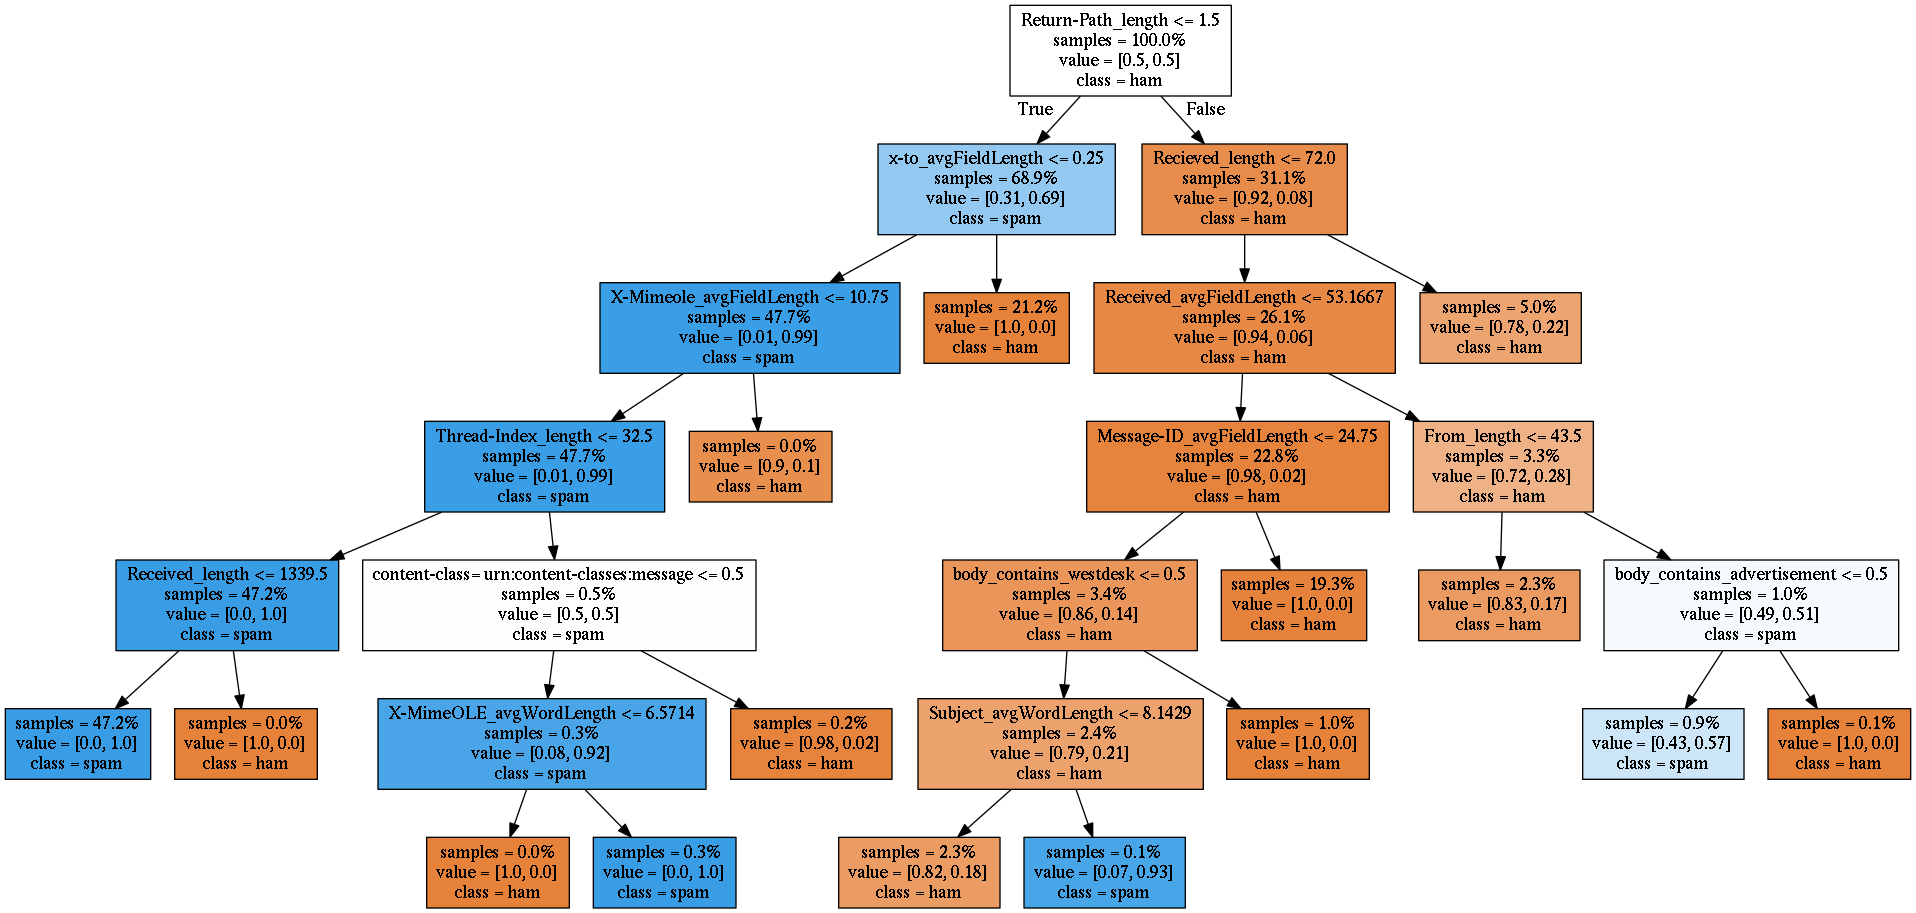
\includegraphics[width=1.3\textwidth]{tree.png}}
	\caption{Árbol de decisión similar con un score un poco menor (pero que es mucho más lindo a la vista).}
\end{figure}

\subsection{Naive Bayes}

Se prueba usar el modelo de Bernoulli usado en sklearn en las variables booleanas del modelo (eso es, todas menos las que hablan de tamaños o de cantidades). Elegimos el parámetro \( \alpha = 1 \) por el simple hecho de que cualquier otro valor daba un peor resultado.

Elegir este modelo aplicando el método de cross validation llega a un score promedio de \( \mathbf{0.952} \).

\section{Reducción de Dimensionalidad}

\section{Resultados}

\section{Discusión}

\end{document}
